Consider the following feedback control system
\begin{center}
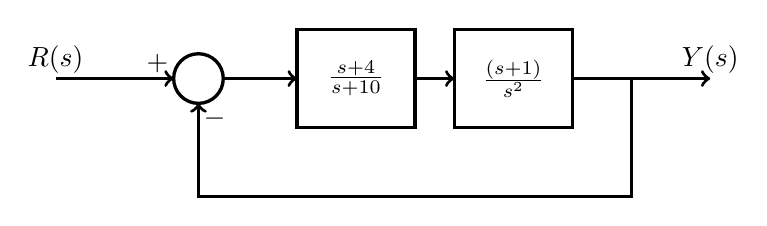
\begin{tikzpicture}[scale=1,inner sep=0pt,outer sep=0pt,very thick,
sysblock/.style={draw,rectangle,inner sep=2pt,minimum width=1.5cm,minimum height=1.25cm,very thick}]
\draw (3,0) node[draw,circle] (sum3) {$\rule{0pt}{18pt}$};
%\draw (7,0) node[draw,circle] (sum2) {$\rule{0pt}{18pt}$};
\draw (7,0) node[sysblock] (G) {$\frac{(s+1)}{s^{2}}$};
\draw (5,-0) node[sysblock] (Kd) {$\frac{s+4}{s+10}$};

\draw[<-] (sum3.180)  node[above left=2pt] {$+$} -- ++(-1.5,0) node[above=2pt] {$R(s)$};
\draw[->] (sum3.0) -- (Kd);
\draw[->] (Kd) -- (G);
\draw[->] (G) -- ++(2.5,0) node[above=2pt] {$Y(s)$};
\draw[->] (G) ++(1.5,0) -- ++(0,-1.5) -| (sum3.-90) node[below right=2pt] {$-$};
%\draw[<-] (sum2.90) node[above right=2pt] {$+$} -- ++(0,1) node[right=2pt] {$D(s)$};
\end{tikzpicture}
\end{center}
Use linear approximation rules to sketch by hand  the Bode plot of the loop gain, and using the information from this plot, sketch the Nyquist plot. Determine if the closed loop system is stable or unstable. The following logscale graph is provided for your convenience.

\includegraphics[width=5in]{\mainfolder/LectureNotes/\lecturefolder/HomeworkProblems/blankbode}
